\documentclass[11pt]{article}


    \usepackage[breakable]{tcolorbox}
    \tcbset{nobeforeafter} % prevents tcolorboxes being placing in paragraphs
    \usepackage{float}
    \floatplacement{figure}{H} % forces figures to be placed at the correct location
    \usepackage{multicol}
	\usepackage[english]{babel}
    \usepackage{tabularx}
    \usepackage{subfigure}
    \usepackage{picture}
    \usepackage{amsmath}
    \usepackage{hyperref}
    \hypersetup{
    colorlinks=true,
    linkcolor=blue,
    filecolor=magenta,      
    urlcolor=cyan,
    }
    \usepackage{graphicx}    
    \usepackage{caption}
    \usepackage{adjustbox} % Used to constrain images to a maximum size 
    \usepackage{xcolor} % Allow colors to be defined
    \usepackage{enumerate} % Needed for markdown enumerations to work
    \usepackage{geometry} % Used to adjust the document margins
    \usepackage{amsmath} % Equations
    \usepackage{amssymb} % Equations
    \definecolor{urlcolor}{rgb}{0,.145,.698}
    \definecolor{linkcolor}{rgb}{.71,0.21,0.01}
    \definecolor{citecolor}{rgb}{.12,.54,.11}
    

    
    % Prevent overflowing lines due to hard-to-break entities
    \sloppy 
    % Setup hyperref package
    \hypersetup{
      breaklinks=true,  % so long urls are correctly broken across lines
      colorlinks=true,
      urlcolor=urlcolor,
      linkcolor=linkcolor,
      citecolor=citecolor,
      }
    % Slightly bigger margins than the latex defaults
    
    \geometry{verbose,tmargin=1in,bmargin=1in,lmargin=0.4in,rmargin=1in}
    \usepackage{fancyhdr}
    \pagestyle{fancy}
    \renewcommand{\footrulewidth}{1pt}
    \rhead{e11921655 Fabian Holzberger \\ e01526208 Jan Ellmenreich}
    \lhead{VU\,184.725\\ High Performance Computing}
    \cfoot{\thepage}
    \setcounter{secnumdepth}{0}
    \setlength\parindent{0pt}

    \usepackage{booktabs}

    \usepackage{listings}
    \usepackage[linesnumbered,ruled,vlined]{algorithm2e}
    \newcommand\mycommfont[1]{\footnotesize\ttfamily\textcolor{blue}{#1}}
    \SetCommentSty{mycommfont}
    \SetKwInput{KwInput}{Input}                % Set the Input
    \SetKwInput{KwOutput}{Output}              % set the Output



\title{Exercise 0 Dataset description}
\author{e12045110 Maria de Ronde \\ eXXXXXXXX  Quentin Andre  \\ e11921655 Fabian Holzberger}
\date{\today}

\begin{document}
\graphicspath{{./figures/}}
\maketitle

\newpage
%
\section{Classification Dataset: Email-Spam (\href{https://www.kaggle.com/nitishabharathi/email-spam-dataset?select=enronSpamSubset.csv}{link to dataset})}


\section{Bridges Dataset(\href{https://archive.ics.uci.edu/ml/datasets/Pittsburgh+Bridges}{link to dataset})}





\section{Kaggle: Amazon review}
\subsection{Dataset Description} 
The Amazon review dataset is a text dataset translated into vectors. There are 50 classes, which represent authors of different reviews. The goal of the classification is to predict the author of reviews. The dataset contains 750 instances with 100002 vectors, a nominal attribute representing a unique ID, 10000 numerical vectors and a nominal vector representing the class.
\newline 
In the figure \ref{Fig::Instances_per_class} below we can see how many instances belong to each class. We can see that the dataset is not balanced. As some classes have 20 instances where other classes have only 10 instances.
\newline
In tabel \ref{Lab::sum_vecs} one can see the distribution of the sum of the vectors. On average a word appears 309 times in all reviews, however there is a word which appears 187520 times, from 49 to 410 times in a review.
%
\begin{figure}[h]
\begin{tabular}{lr}
\toprule
{} &              0 \\
\midrule
count &   10000.000000 \\
mean  &     308.859700 \\
std   &    2419.468303 \\
min   &       0.000000 \\
25\%   &       9.000000 \\
50\%   &      21.000000 \\
75\%   &     220.000000 \\
max   &  187520.000000 \\
\bottomrule
\end{tabular}
\caption{Distribution sum of vectors}
\label{Lab::sum_vecs}
\end{figure}
%
\begin{figure}[h]
\begin{picture}(400,285)
\put(0,0){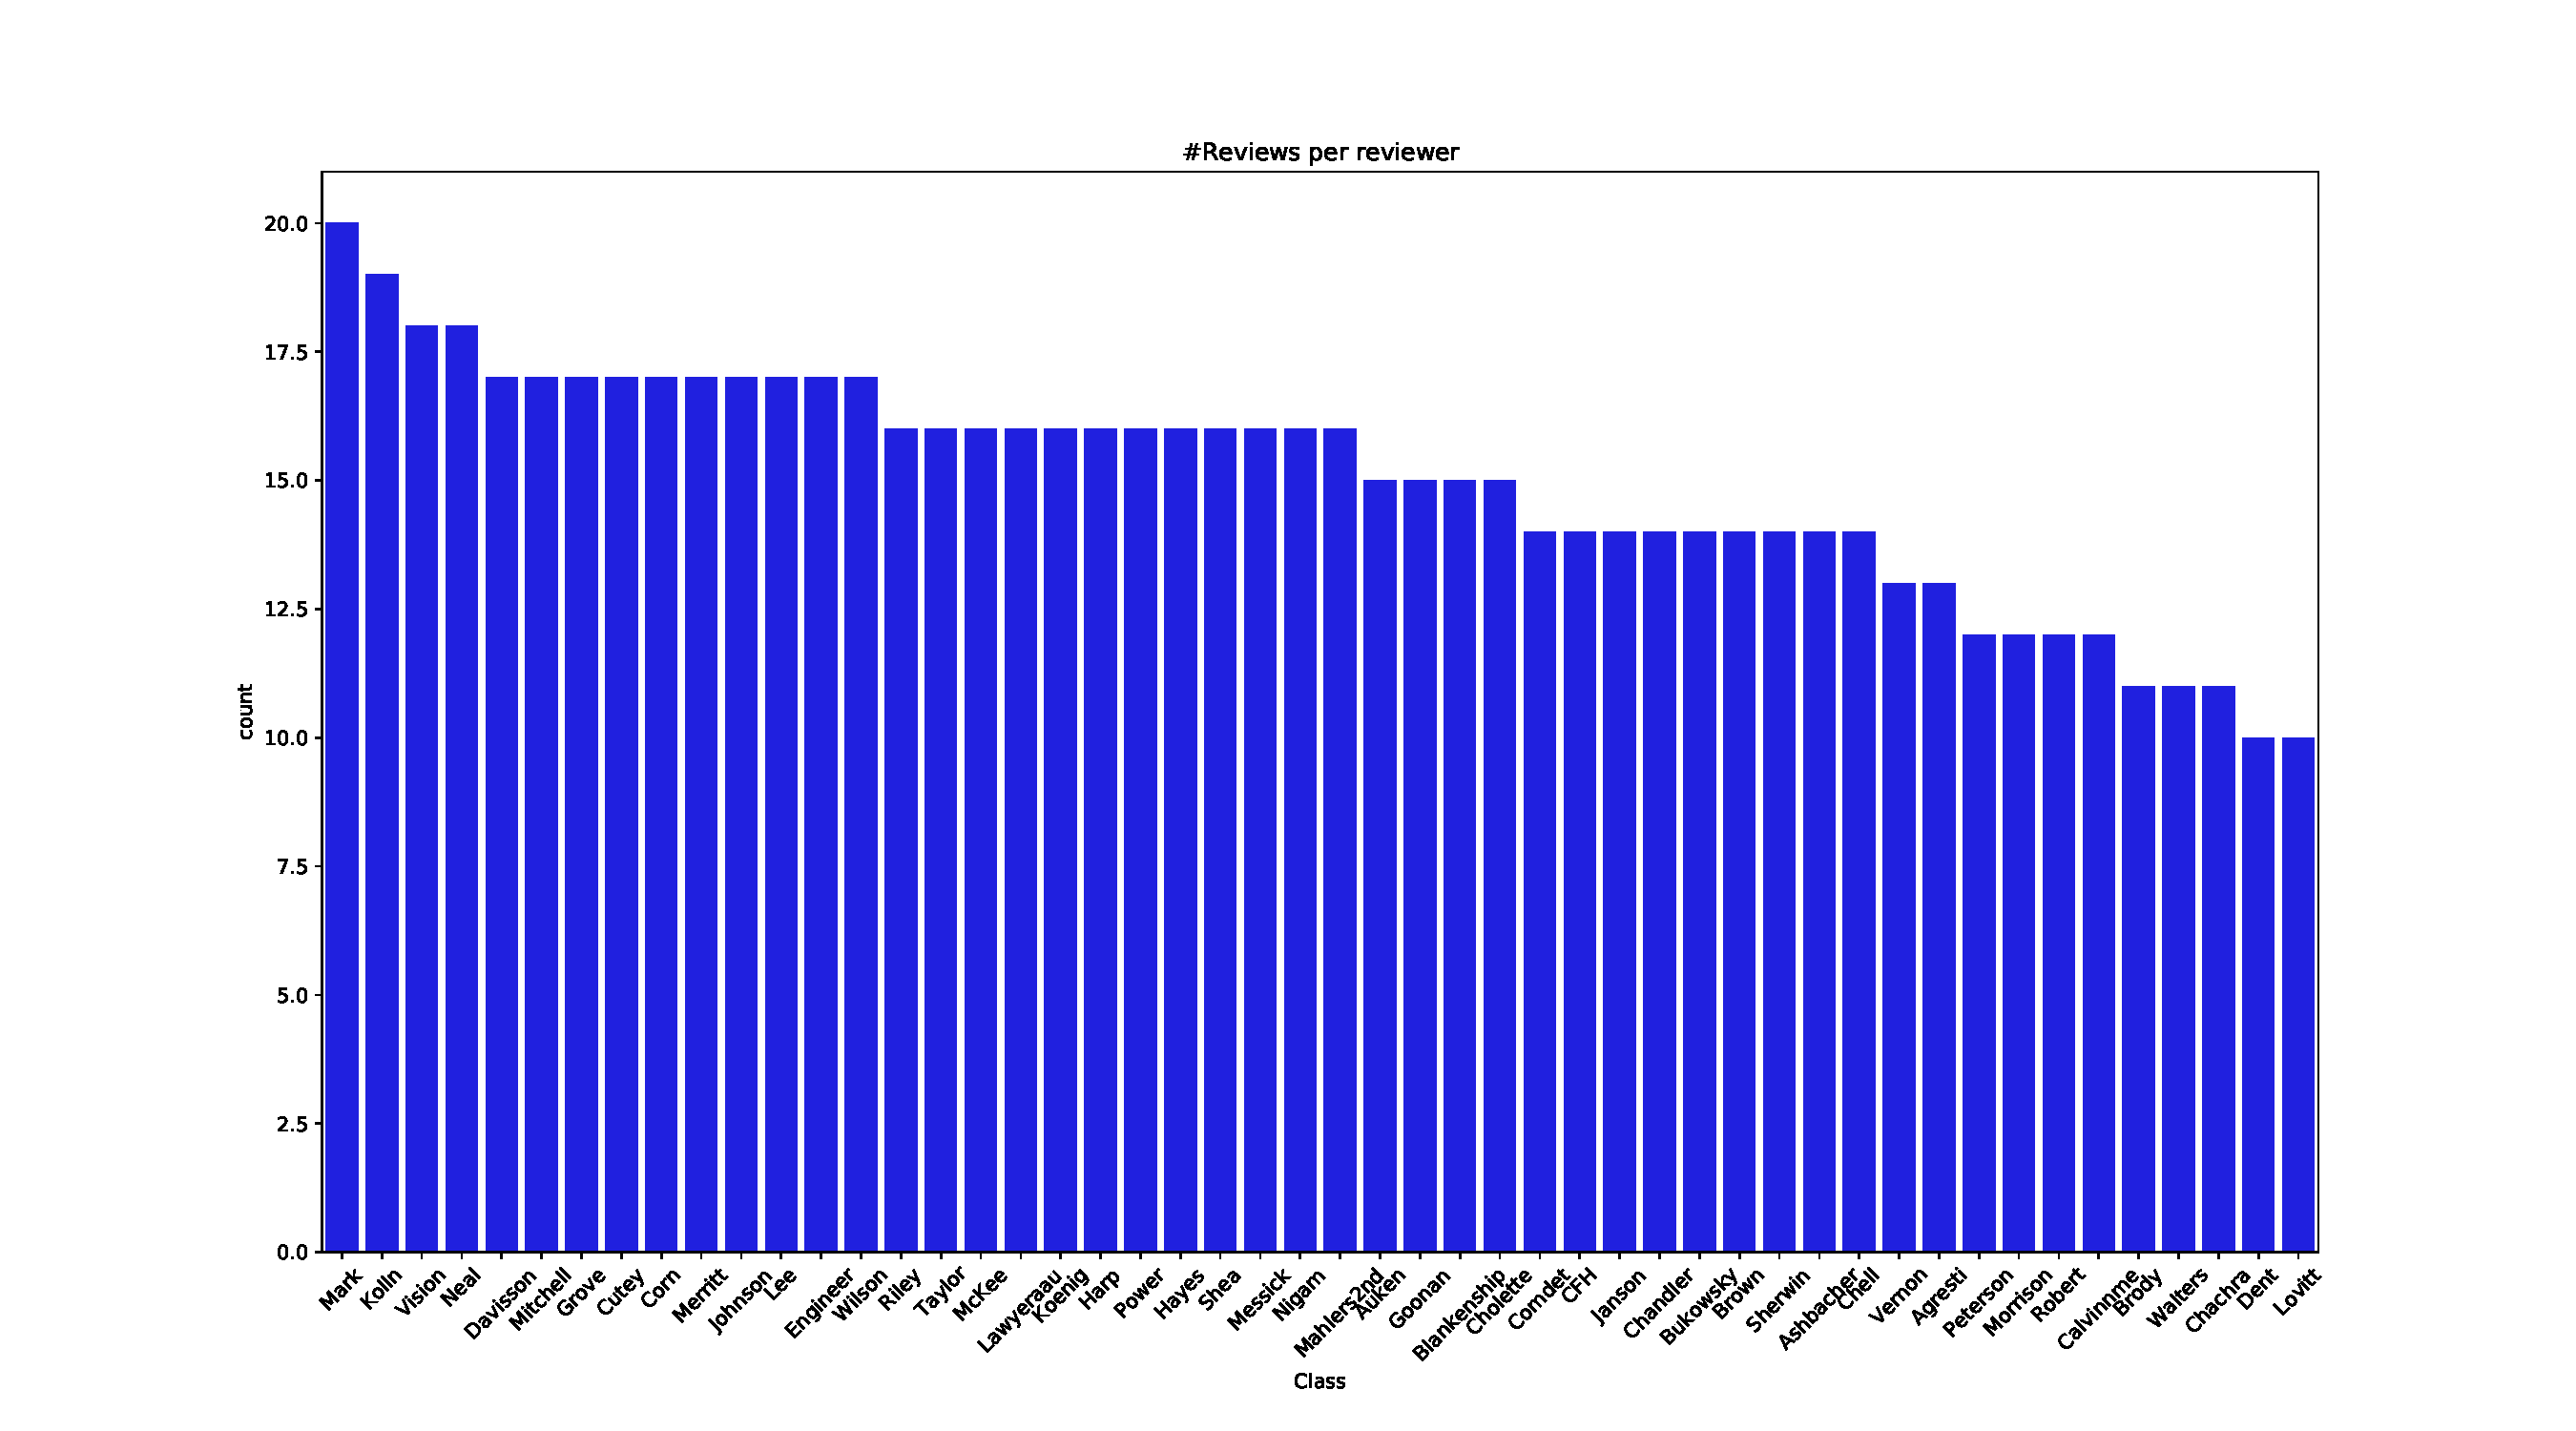
\includegraphics[width=1.00\linewidth]{Instances_per_class.pdf}}
\end{picture}
\caption{Instances per class}
\label{Fig::Instances_per_class}
\end{figure}
%
\subsection{Pre-Processing}
There are no missing values in the dataset. The unique ID has been deleted from the data set as has no relevance to the class. The text vectors have values differentiating of a mean of 250 occurrences per instance to 1 occurrence in the entire dataset. With 250 occurrences per instance it appears as though stop words have not been deleted from the dataset, however as we do not have the raw data available we cannot be certain. 
\newline
We sort the vectors from highest number of total occurrences to the smallest number of total occurrences. Words which only occur in one instance can be seen as unique identifier to one author.
By sorting the data we enable, to train our model  leaving some of the first and last columns out and test whether this improve the model.
\newline
In tabel X one can see the distribution of the sum of the vectors. On average a word appears 309 times in all reviews, however there is a word which appears 187520 times, from 49 to 410 times in a review.
\newline
In order to flatten the weight of words which occur more often in one instance we will also train the model on the natural logarithm of the original dataset. The dataset will be transferred into $ln(X)+1$.
\begin{tabular}{lr}
\toprule
{} &	Sum of vector \\
\midrule
count &   10000.000000 \\
mean  &     308.859700 \\
std   &    2419.468303 \\
min   &       0.000000 \\
25\%   &       9.000000 \\
50\%   &      21.000000 \\
75\%   &     220.000000 \\
max   &  187520.000000 \\
\bottomrule
\end{tabular}

\begin{tabular}{lll}
\toprule
{} &   Scenario &  Scenario description \\
\midrule
0 &      10000 & Select all 10000 attributes   \\
1 &       8000 & select the first 8000 attributes  \\
2 &       6000 & select the first 6000 attributes   \\
3 &   50:10000 & select the 50th till the 10000th attribute   \\
4 &    50:8000 & select the 50th till the 8000th attribute    \\
5 &    50:6000 & select the 50th till the 6000th attribute    \\
6 &  100:10000 & select the 100th till the 10000th attribute    \\
7 &   100:8000 & select the 100th till the 8000th attribute    \\
8 &   100:6000 & select the 100th till the 6000th attribute	\\ 
\bottomrule
\end{tabular}

We create 9 scenarios, which are shown in table X for which we train the three classifiers: Perceptron, Random forest and Naive Bayes with the multi-nominal distribution.   


text
\subsection{Parameter-Tuning}
First we will split the data in two parts. One part for training the model and one part for validating the models afterwards, we use the hold out strategy here. The training dataset is split into a training and test set, this is done with the hold out strategy as well as the cross validation. The results of the model on the test sets are used to tune the parameters on the model.

\subsection{Perceptron}
We determine the base parameters for the perceptron, alpha as 0.0005, eta as 1 penalty='none' and the max iterations are equal to 100. 
\newline
All train set of the $ln(X)+1$ have an accuracy of a 100, for $X$, we could not obtain a perfect score when high occurring words were deleted. 
Comparing the accuracy of the test set of $X$ to $ln(X)+1$,we see that the logarithmic dataset performs better when we do not delete the words with high occurrences. After removing the top 100 words the accuracy of the $X$ dataset is higher than the$ln(X)+1$ dataset. Taking the logarithmic values has the highest effect on the words which occur most often.
\newline
A clear difference can be seen between the performance of the hold out and the cross validation runs. The cross validation run clearly out performs the hold out run. Due to the high amount of classes, 50, and the relative low amount of instances it can happen that classes are not represented in the test set, some classes only appear 10 times in the entire dataset. The accuracy is sensitive to the chosen test and train set. With using the cross validation the entire dataset is used and the influence of chance decreases. In order to the hyper parameters we will use cross validation and look at the results of the test set. For the parameter tuning scenario 4 of the unstransformed dataset is chosen. Scenario performed slightly better. The vectors with very low occurrences might have unique identifiers to classes, which increases over fitting. 
\newline
Overfitting....??? What to do
   
\begin{tabular}{llrrrr}
\toprule
{} &   Scenario &  Basic test &  Basic train &    LN test &  LN train \\
\midrule
0 &      10000 &   37.777778 &    91.666667 &  40.000000 &     100.0 \\
1 &       8000 &   39.259259 &    91.296296 &  41.481481 &     100.0 \\
2 &       6000 &   40.000000 &    88.148148 &  47.407407 &     100.0 \\
3 &   50:10000 &   40.740741 &   100.000000 &  34.074074 &     100.0 \\
4 &    50:8000 &   40.740741 &   100.000000 &  36.296296 &     100.0 \\
5 &    50:6000 &   40.000000 &   100.000000 &  41.481481 &     100.0 \\
6 &  100:10000 &   40.000000 &   100.000000 &  43.703704 &     100.0 \\
7 &   100:8000 &   40.000000 &   100.000000 &  42.962963 &     100.0 \\
8 &   100:6000 &   37.037037 &   100.000000 &  41.481481 &     100.0 \\
\bottomrule
\label{tab:Accuracy perceptron hold out}
\end{tabular}

\begin{tabular}{llrrrr}
\toprule
{} &   Scenario &  Basic test &  Basic train &    LN test &  LN train \\
\midrule
0 &      10000 &   40.133333 &    93.229630 &  50.133333 &     100.0 \\
1 &       8000 &   40.000000 &    93.585185 &  50.266667 &     100.0 \\
2 &       6000 &   39.466667 &    92.340741 &  51.200000 &     100.0 \\
3 &   50:10000 &   51.600000 &   100.000000 &  50.666667 &     100.0 \\
4 &    50:8000 &   51.200000 &   100.000000 &  50.266667 &     100.0 \\
5 &    50:6000 &   49.066667 &   100.000000 &  50.400000 &     100.0 \\
6 &  100:10000 &   50.800000 &   100.000000 &  49.333333 &     100.0 \\
7 &   100:8000 &   50.533333 &   100.000000 &  50.133333 &     100.0 \\
8 &   100:6000 &   50.266667 &   100.000000 &  48.933333 &     100.0 \\
\bottomrule
\label{tab:Accuracy perceptron cross validation}
\end{tabular}

\subsubsection{Parameter tuning}
The first parameter we tune is the maximum number of iteration $max_iter$. We test for values $ max_iter \in \{2, 3, 4, 5, 10, 50, 100\}$. It can be seen that after 10 iterations the training set has a perfect fit, and the test set has the highest accuracy, as well as precision and recall. Therefore, we take $max_iter=10$ for the next parameter test.
\newline
Following the model has been ran for different learning rates ($eta0$), where $ eta0 \in \{1^-4, 1^-3, 0.01, 0.1, 0.2, 0.3, 0.4, 0.6, 0.8, 1\} $. The model is indifferent for the learning rate and always obtains the same accuracy, precision and recall values. This means that the same weights are obtained.
\newline
Since the model is over fitting a regularization term has been introduced. At first $\alpha$ was set to be $ \in \{1^-4, 1^-3, 0.01, 0.5, 1\}$. The accuracy for both the training set as well as the test set dropped rapidly after $1^-3$. Therefore, a second run with $\alpha \in  \{1e-5, 1e-4, 0.0002, 0.0004, 0.0006, 0.0008, 1e-3\}$ has been done. For $\alpha=0.0002$, the test set performs best with $49.16\%$. 

\begin{tabular}{lrrr}
\toprule
{} &  Scenario &  Basic test &  Basic train \\
\midrule
0 &   0.00001 &   47.258560 &   100.000000 \\
1 &   0.00010 &   47.532924 &    99.983526 \\
2 &   0.00020 &   49.163740 &    99.473169 \\
3 &   0.00040 &   41.922739 &    98.616470 \\
4 &   0.00060 &   39.078139 &    94.471517 \\
5 &   0.00080 &   41.027217 &    96.558869 \\
6 &   0.00100 &   42.811677 &    96.806311 \\
\bottomrule
\label{Accuracy testing for alphas}
\end{tabular} 

\subsubsection{Validation}
Finally we run our final model with the following parameter settings, maximum number of iterations is 10, $eta0=1$, the regularization term is l1, with an $\alpha$ of $0.0002$ against the validation set. This results in an accuracy of $50.4\%$. In the confusion matrix we can see that some names are never predicted and some names are predicted too often, like Brown. 
%
%
\subsection{Random forest}
The second classifier is the random forest classifier. First it is checked which data pre-process steps will be applied to the model. The base parameter settings are the following:
$ccp \alpha = 0$ \\
$max leaf = 50$ \\
$max depth = 10$ \\
$number of estimators = 100$\\
The best scenario is scenario 1 on the natural logarithmic dataset with and accuracy of $49.17\%$ in the cross validation. This model is less sensitive for the extreme values of words with an high occurrence as the results of $X\%$ and $LN(X)+1$ are closer to each other, as well as the model taking the first attributes into account scoring highest on accuracy. Using cross validation the $LN(X)+1$ always out performs the dataset $X$, where in the hold out run there is not pattern to be seen. 
\newline
The following hyper parameters have been tested: number of estimators, the maximum depth, maximum leafs and the ccp alpha. Starting with the number of estimators, also the number of trees, given n estimators $\in \{1,5,10,50,70, 100, 200\}$. 
\newline
Both the train set and the test set achieve an higher accuracy whenever the number of estimators increases. The number of estimators will be set to 200.
The second hyper parameter is the maximum number of leafs per branch, we test $max leafs \in \{5,10, 20, 50, 100\}$ The accuracy increases when the number of leafs increase to 50, with 100 the accuracy, precision and recall do increase for the training set, but not for the test set. The maximum number of leafs is set to 50.   
\newline
After the number of trees and the leafs per branch, the depth of each tree is determined. where $max depth \in \{2, 3, 4, 5, 8, 10, 50, 100\}$. The accuracy for the training set is highest with a maximum depth of $10$. The accuracy for the test set is highest with a maximum depth of $50$ or a $100$, the same scores are obtained. The maximum depth is set to $50$. 
\newline
Finally we will include some minimal cost complexity pruning. We test for $ccp  \alpha \in \{1e-5, 2e-5, 1e-4, 2e-4, 1e-3, 5e-3, 75e-4, 1e-2\}$. It can be seen that for $ccp \alpha < 0.005$ no pruning has been done. However, for $ccp \alpha > 0.005$ both the train and the test have reduced scores. Therefor, we will set $ccp \alpha=0.005$.   
%
\newline
\begin{tabular}{llrrrr}
\toprule
{} &   Scenario &  Basic test &  Basic train &    LN test &    LN train \\
\midrule
0 &      10000 &   42.222222 &    99.814815 &  43.703704 &   99.814815 \\
1 &       8000 &   39.259259 &    99.814815 &  39.259259 &   99.814815 \\
2 &       6000 &   39.259259 &    99.814815 &  38.518519 &   99.814815 \\
3 &   50:10000 &   37.037037 &    99.814815 &  37.777778 &   99.814815 \\
4 &    50:8000 &   37.777778 &   100.000000 &  36.296296 &  100.000000 \\
5 &    50:6000 &   41.481481 &    99.814815 &  38.518519 &   99.814815 \\
6 &  100:10000 &   37.037037 &    99.629630 &  36.296296 &   99.629630 \\
7 &   100:8000 &   35.555556 &    99.444444 &  34.814815 &   99.444444 \\
8 &   100:6000 &   37.037037 &    99.444444 &  37.777778 &   99.444444 \\
\bottomrule
\label{Random forest hold out}
\end{tabular}
\newline
\begin{tabular}{llrrrr}
\toprule
{} &   Scenario &  Basic test &  Basic train &    LN test &   LN train \\
\midrule
0 &      10000 &   46.222564 &    99.703812 &  46.808604 &  99.720259 \\
1 &       8000 &   48.432836 &    99.703731 &  49.174715 &  99.736652 \\
2 &       6000 &   46.804214 &    99.868340 &  47.098332 &  99.851892 \\
3 &   50:10000 &   47.245391 &    99.325143 &  47.396839 &  99.341618 \\
4 &    50:8000 &   45.037313 &    99.489644 &  45.041703 &  99.506145 \\
5 &    50:6000 &   46.661545 &    99.720286 &  47.695347 &  99.720286 \\
6 &  100:10000 &   45.610184 &    99.193429 &  46.341089 &  99.176954 \\
7 &   100:8000 &   46.501317 &    99.226215 &  46.652766 &  99.226215 \\
8 &   100:6000 &   44.721247 &    99.374404 &  44.725637 &  99.374404 \\
\bottomrule
\label{Random forest cross validation}
\end{tabular}
\subsubsection{Validation}
The final model is now tested on the validation data with the following parameter settings:
$ccp \alpha = 0.005$ \\
$max_leaf = 50$ \\
$max_depth = 50$ \\
$n estimators = 200$ \\ 
This gives a accuracy of 
 
 \subsection{Performance-Analysis}
\end{document}


